\section{Statistics for Beginner's Algorithm}
\label{sec:beginnersStat}
In order to get the average length of a solution of beginner's algorithm we must determine how many moves of scrambling must be applied in order to find the worst case scenario. 
By computing the average for different amount of scrambles the graph quickly becomes steady at around 40 scrambles (10.000 cubes is tested) (see figure \ref{fig:beginnersScramble}). To be sure that we get a good result we go by 50 scrambles.
\begin{figure}[htbp]
	\centering
		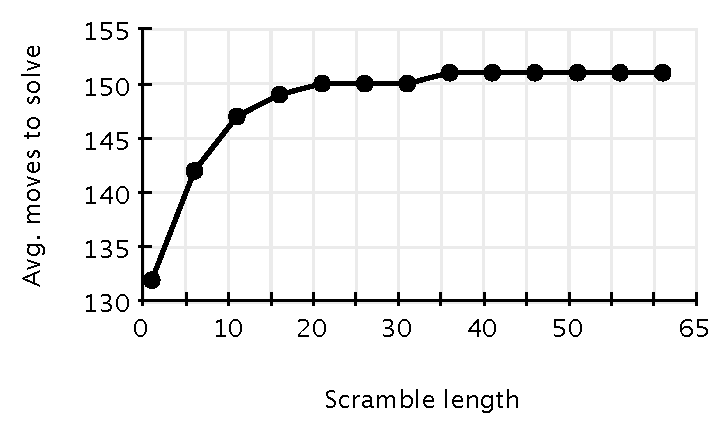
\includegraphics{input/pics/beginnersScramble.pdf}
	\caption{\myCaption{The graph shows the amount of moves needed to solve a cube with x scrambles. The lines are for showing only and do not represent the average between the dots.}}
	\label{fig:beginnersScramble}
\end{figure}

Now that the number of scrambles is determined the average number of \twist{}s can be found.
By scrambling 10 million \cube{}s and solve them with the beginner's algorithm we get an average of \textbf{151 moves}.
A test using only 1 million \rubik{}s is run three times in order to insure that the test is reliable.
The raw data from both tests is found in appendix \ref{chap:beginnerResults}.
%Which is the average of beginner's algorithm.
The maximum value found is 241 moves and minimum is 56 moves.
The average time spend on each solve was:
\[
\frac{502552ms+490385ms+498937ms+4734126ms}{10^{7} + 3 \cdot 10^{6}} = 0,478923077ms
\]

The data was gathered on a computer operated by Windows 7 64 bits running on a 2.5 GHz AMD Quad Core processor (905e) with 4 GB DDR-3 RAM.

A peculiar note is that with one twist scramble, the algorithm needs an average of 132 moves with a maximum of 155 and a minimum 94 moves to solve it again.
This illustrates the twist-wise inefficiency of this algorithm very well.
